\setAuthor{EFO žürii}
\setRound{lahtine}
\setYear{2016}
\setNumber{G 1}
\setDifficulty{2}
\setTopic{Dünaamika}

\prob{Mängukahur}
\begin{wrapfigure}[6]{r}{0.4\textwidth}
 \vspace{-20pt}
 \begin{center}
 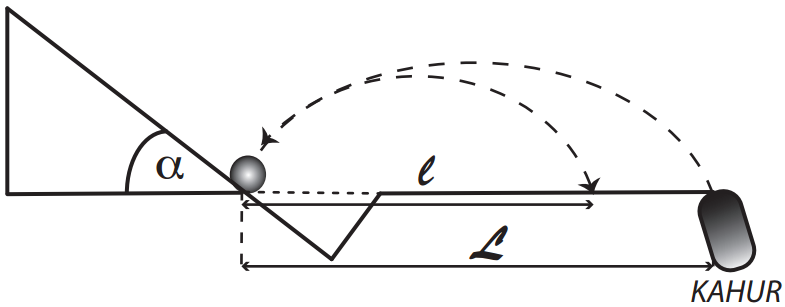
\includegraphics[width=0.4\textwidth]{2016-lahg-01-kaldjoonis}
 \end{center}
 \vspace{-30pt}
\end{wrapfigure}

Mängukahurist tulistatakse kummipall nii, et see põrkab risti kaldpinnaga, kahurist horisontaalkaugusel $L$. Pall põrkab kaldpinnast tagasi kaugusele $l$ (vt joonis). Leidke, kui suur osa energiast neeldus põrkel. Kaldpinna kaldenurk on $\alpha$.

\hint
Kuna pall maandub kaldpinnale risti, siis liigub pall sellel hetkel nurgaga $\alpha$ vertikaali suhtes. Seega tulistatakse pall kahurist välja samuti nurga $\alpha$ all vertikaali suhtes ning pall põrkab kaldpinnalt tagasi sama nurga all.

\solu
Kuna pall maandub kaldpinnale risti, siis liigub pall sellel hetkel nurga $\alpha$ all vertikaali suhtes. Seega tulistatakse pall kahurist välja ka nurga $\alpha$ all vertikaali suhtes ning pall põrkab kaldpinnalt tagasi ka sama nurga all. Palli horisontaalne kiiruse komponent on $v\sin(\alpha)$ ja vertikaalne komponent on $v\cos(\alpha)$. Trajektoori kõige ülemises punktis on vertikaalne kiiruse komponent null ja on kulunud pool kogu liikumise ajast $t$. Aja $t/2$ jooksul muutub kiirus raskuskiirenduse tõttu $gt/2$ võrra, seega $gt/2 =v\cos(\alpha)$, millest $t=2v\cos(\alpha)/g$. Horisontaalne kiirus ei muutu liikumise jooksul. Horisontaalselt läbitud vahemaa on $$s=vt\sin(\alpha)=\frac{2v^2\cos(\alpha)\sin(\alpha)}{g} = \frac{v^2\sin(2\alpha)}{g}.$$
Seega kahurist tulistades oli palli algkiirus $v_1$, kus
\[ v_1^2 = \frac{Lg}{\sin(2\alpha)}, \]
ning tagasipõrkel $v_2$, kus
\[ v_2^2 = \frac{lg}{\sin(2\alpha)}. \]
Tulistamise ja tagasipõrkamise hetkel oli pallil ainult kineetiline energia:
\[ E_1 = \frac{mv_1^2}{2}=\frac{mLg}{2\sin(2\alpha)},\quad\quad E_2 =\frac{mv_2^2}{2} = \frac{mlg}{2\sin(2\alpha)}. \]
Seega põrkel kaduma läinud energia osakaal on
\[ \frac{E_1-E_2}{E_1} = \frac{L-l}{L}. \]

\probeng{Toy cannon}
\begin{wrapfigure}[8]{r}{0.5\textwidth}
  \vspace{-20pt}
  \begin{center}
    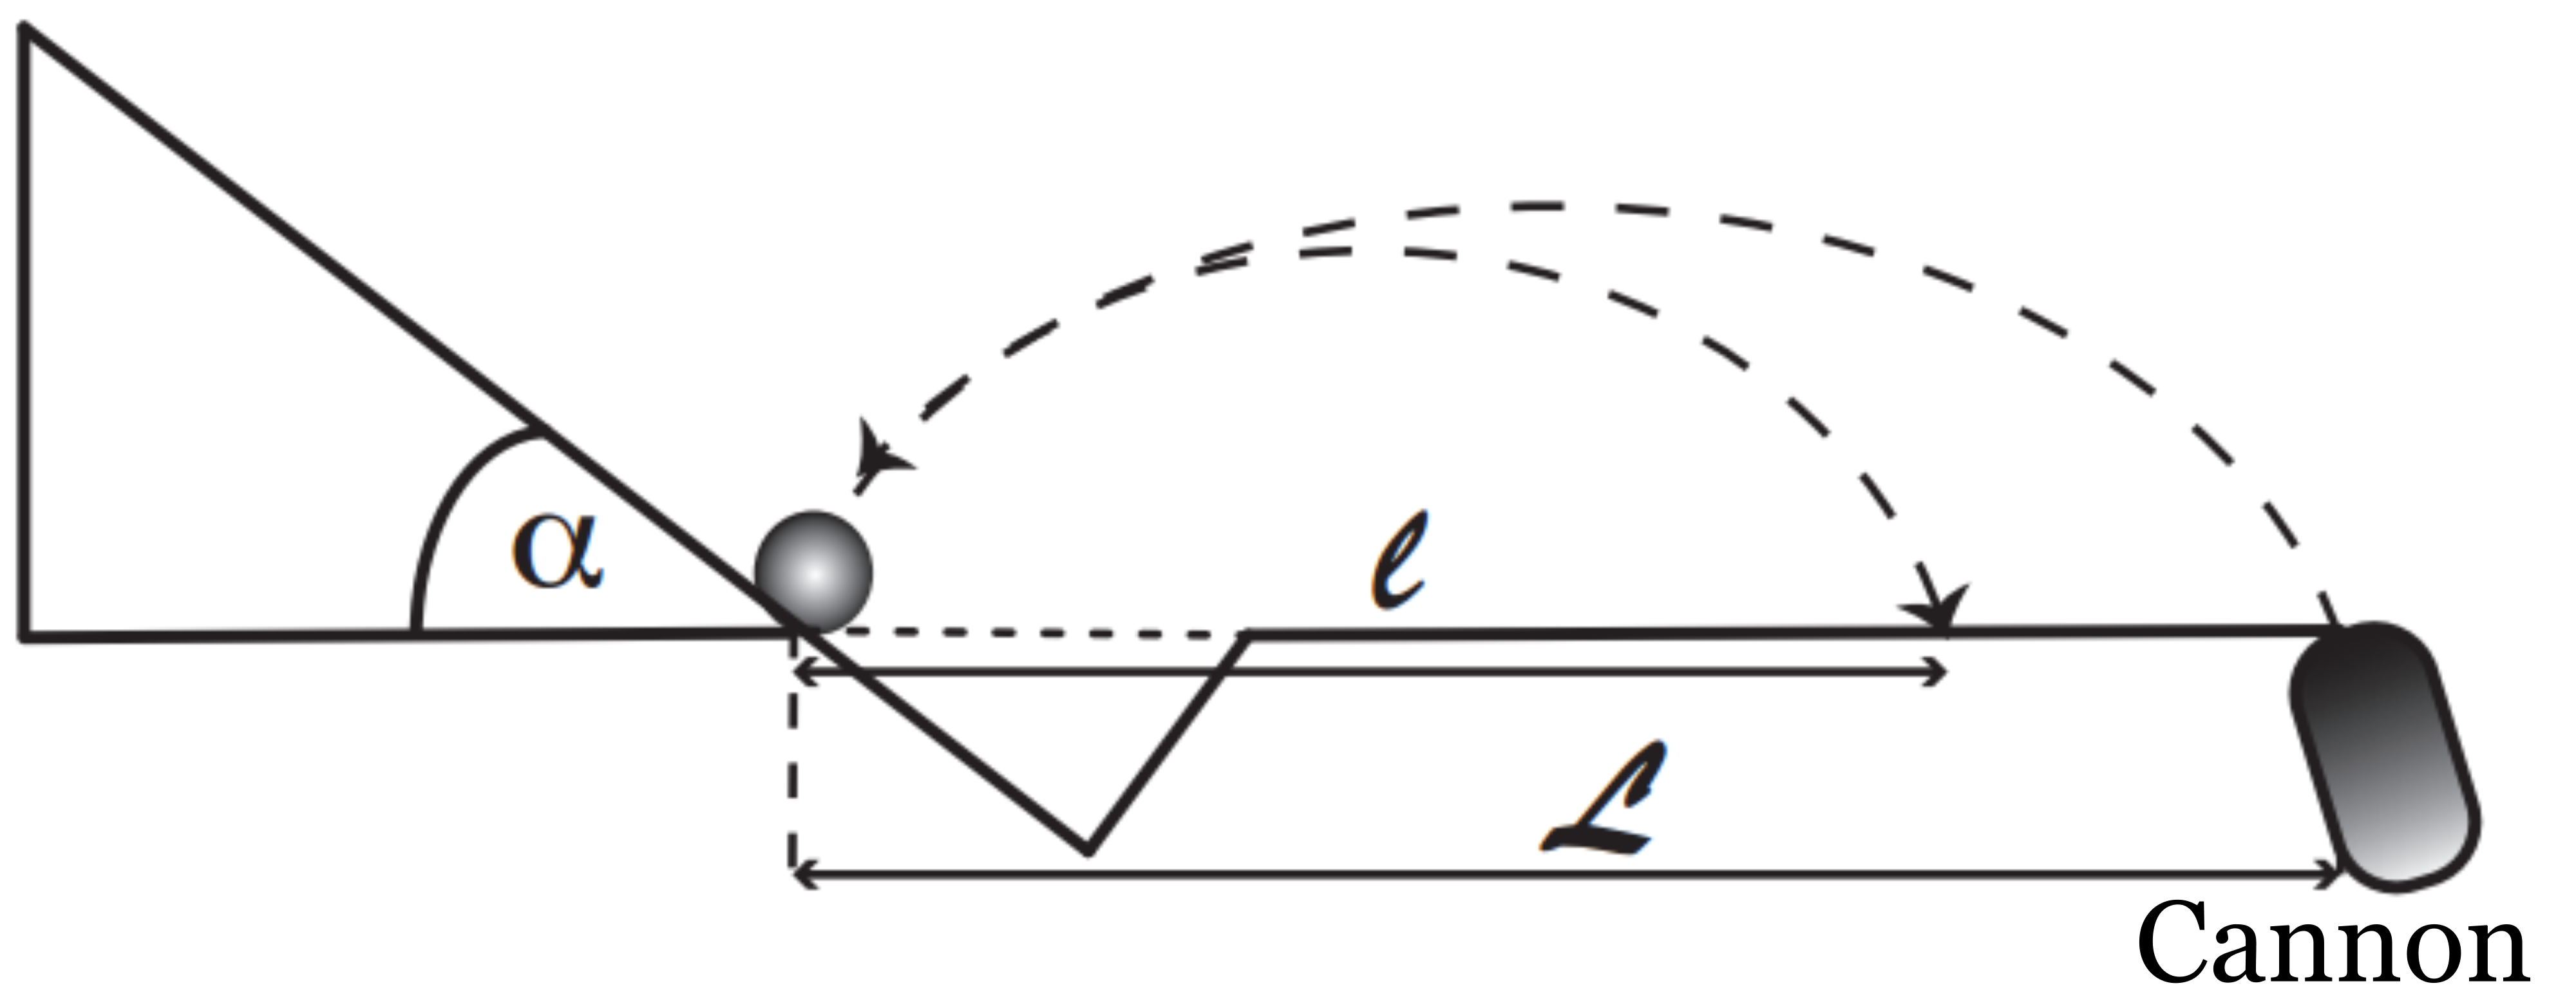
\includegraphics[width=0.5\textwidth]{2016-lahg-01-kaldjoonis_ing}
  \end{center}
  \vspace{-30pt}
\end{wrapfigure}
A rubber ball is fired out of a toy cannon so that the ball bounces perpendicularly to an inclined surface distanced horizontally $L$ from the cannon. The ball bounces off from the inclined surface to a distance $l$ (see figure). Find what fraction of the energy got absorbed during the bounce. The surface’s angle of inclination is $\alpha$.

\hinteng
Because the ball lands perpendicularly to the inclined surface then at this moment the ball moves at the angle $\alpha$ with respect to the vertical. Thus the ball is fired out of the cannon also at the angle $\alpha$ with respect to the vertical and then the ball bounces back from the inclined surface at the same angle.

\solueng
Because the ball lands perpendicularly to the inclined surface then the ball moves at the angle $\alpha$ with respect to the vertical at this moment. Thus the ball is shot out of the cannon also at the angle $\alpha$ with respect to the vertical and the ball bounces back from the inclined surface at the same angle as well. The horizontal velocity component of the ball is $v\sin(\alpha)$ and the vertical component $v\cos(\alpha)$. At the uppermost point of the trajectory the vertical component of the velocity is zero, at which moment half of the total time of movement $t$ has passed. During the time $t/2$ the velocity changes due to the gravitational acceleration by $gt/2$, thus $gt/2 =v\cos(\alpha)$, where $t=2v\cos(\alpha)/g$. The horizontal velocity does not change during the motion. The distance covered horizontally is
$$s=vt\sin(\alpha)=\frac{2v^2\cos(\alpha)\sin(\alpha)}{g} = \frac{v^2\sin(2\alpha)}{g}.$$ 
Thus, when firing from the cannon the initial velocity of the ball was $v_1$ where
\[ v_1^2 = \frac{Lg}{\sin(2\alpha)}, \] 
and when bouncing back $v_2$ where
\[ v_2^2 = \frac{lg}{\sin(2\alpha)}. \] 
At the moment of firing and bouncing back the ball only had kinetic energy:
\[ E_1 = \frac{mv_1^2}{2}=\frac{mLg}{2\sin(2\alpha)},\quad\quad E_2 =\frac{mv_2^2}{2} = \frac{mlg}{2\sin(2\alpha)}. \]
Thus, the fraction of the energy lost during the bounce is
\[ \frac{E_1-E_2}{E_1} = \frac{L-l}{L}. \]
\probend